The graphical user interface (GUI) is called a timeline (see Figure \ref{GoogleGlassUI}). The timeline consists of a row of cards. Cards are basic applications such as a clock or information about the weather. Cards can also represent more in-depth applications, on Google Glass called ``Immersions''. An immersion handles activities such as browsing an image gallery or playing a game.\\

WRITE ABOUT HOME SCREEN (CLOCK; CAN BE STARTED WITH "OK GLASS"

	\begin{figure}[ht!]
		\centering
		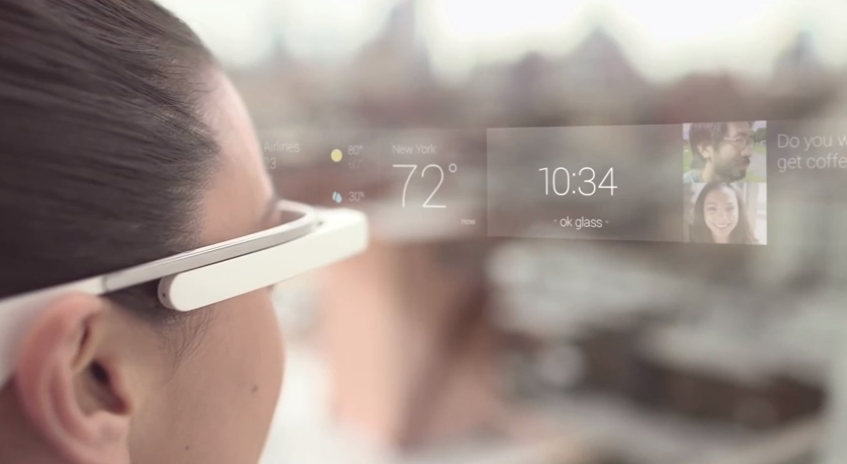
\includegraphics[width=110mm]{images/GoogleGlassUI}
		\caption{A virtual representation of the Google Glass user interface as the graphical user interface is perceived by the user.\cite{ImagesGoogleGlassUI}}
		\label{GoogleGlassUI}
	\end{figure}

On the timeline cards to the left of the home screen are upcoming activities such as an event in the user's calendar or an upcoming flight. Cards to the right of the home screen are from the past. Cards from the past will for instance show text messages or photos. When the user wants to turn of Google Glass the user swipes down on the touchpad. Swiping down on the touchpad will put Google Glass in stand by. If the user wants to turn of Google Glass entirely there is a power button on the opposite side of the touchpad. Holding down the power button for a few seconds will turn of Google Glass. For a better visual understanding of how Google Glass works see Figure \ref{GoogleGlassUI} as well as the video referenced in the caption.\\



%The main way for a user to give input to Google Glass is via the touchpanel that is mounted on the right hand side of Glass, along the frame. Users are able to swipe as well as tap, which gives them control similar to that of a Smart TV's user interface. Where with a TV controller the user would maneuver with a simple cross layout (up, down, right and left) the buttons have on Glass been replaced by a touchpanel.\\

% Insert image of Google Glass graphical user interface here!!!

%The graphical interface is displayed at the top right through a projection coming from the right on a thick piece of glass. This technique lines up the image with the users sight but does not give any projection outwards.\\

%The interface is built with cards. Each card represents an activity.\\

%What’s unique?
%Standards?
%\url{https://developers.google.com/glass/design/}